%--------------------------- IMPORTS AND SETTINGS -----------------------------

\documentclass[12pt]{article}

\usepackage[a4paper,
inner  = 25mm,
outer  = 25mm,
top    = 25mm,
bottom = 25mm]{geometry}

\usepackage{lmodern}
\usepackage[english]{babel}
\usepackage[utf8]{inputenc}
\usepackage[T1]{fontenc}
\usepackage[hidelinks]{hyperref}
\usepackage{graphicx}
\usepackage{amssymb}
\usepackage{amsmath,tabu}
\usepackage{epstopdf}
\usepackage[nottoc,numbib]{tocbibind}
\usepackage{setspace}
\usepackage[none]{hyphenat}
\usepackage[justification=centering]{caption}

\usepackage{url}
\PassOptionsToPackage{hyphens}{url}\usepackage{hyperref}

\setstretch{1.2}

\begin{document}

%-------------------------------- TITLE PAGE ----------------------------------

\begin{titlepage}
	\vspace*{0cm}
	\centering
	\begin{tabular}{cp{1cm}c}
		\begin{minipage}{4cm}
			\vspace{0pt}
			
\includegraphics[width=1\textwidth]{images/elte_logo.png}
		\end{minipage} & &
		\begin{minipage}{7cm}
			\vspace{0pt}Eötvös Loránd Tudományegyetem \vspace{10pt} \newline
			Informatikai Kar \vspace{10pt} \newline
			Komputeralgebra Tanszék
		\end{minipage}
	\end{tabular}

	\vspace*{0.2cm}
	\rule{\textwidth}{1pt}

	\vspace*{3cm}
	{\Huge Modelling and testing}

	\vspace*{0.5cm}
	{\normalsize IPM-18EszKVMTEG}

	\vspace{2cm}
	{\huge A model based approach to testing Neovim's mode transitions}

	\vspace*{5cm}

	{\large \verb|Zahorán Barnabás| }

	{\large \verb|idggb6@inf.elte.hu| }

	\vfill

	\vspace*{1cm}
	\today
\end{titlepage}


%----------------------------- TABLE OF CONTENTS ------------------------------

\tableofcontents
\cleardoublepage


%----------------------------------- MAIN ------------------------------------

\section{Abstract}
	Modal text editors, like Vi and its derivatives, support different editing modes, each based around distinct tasks and each having a different set of keybindings. Reusing keys like this leads to a more efficient text editing workflow by decreasing the number of keystrokes required for frequent editing tasks. It is important for the modes and the transitions between them to be well defined and consistent. This study aims to present a model based approach to generating testcases that can verify the text mode transitions of Neovim.
	\\
	\\
	Keywords: Neovim, nvim, modal editor, FSM, model based testing, test generation

\section{Glossary}
	nvim: Neovim (nvim is the name we can use on the command-line to launch it)\\
	mode: Editing mode of Neovim\\
	FSM: Finite State Machine\\
	MBT: Model-Based Testing\\
	MTR: Model >> Test >> Relax MBT framework\\
	TSV: Tab Separated Values text format\\
	TT: Transition Tour MBT method\\
	ATS: All-Transition-State MBT method\\
	\verb|<Esc>|: nvim's notation for the Escape key\\
	\verb|<Ins>|: nvim's notation for the Insert key\\
	\verb|<CR>|: nvim's notation for the Enter key (CR stands for Carriage Return)\\
	\verb|<C-c>|: nvim's notation for the CTRL-c key combination

\section{Introduction}

	\subsection{System under test}

		Neovim \cite{nvim} is a fork and modernized version of Vim which itself is an ascendant of the Unix visual text editor Vi. They all support modal text editing and all Unix or Unix-like systems ship with at least Vi installed since about the seventies.

		The program starts in \verb|Normal| mode, where the user can navigate the cursor, search text or initiate a number of different text input commands. In the latter case, the editor prompts the user to enter text into the visual buffer. This is called \verb|Insert| mode. \verb|Visual|, \verb|Visual line| and \verb|Visual block| modes allow the user to select sections of the text. \verb|Cmdline| allows us to run Vim commands, while \verb|Ex| mode lets us issue legacy ex commands.

		These are only a small portion of all modes. To get a complete list that also includes more obscure ones such as the different \verb|Operator-pending| modes, run \verb|:help mode()| in nvim.

		The user can switch between these modes using certain keys, e.g. from \verb|Normal| the \verb|i| key takes us to \verb|Insert| and \verb|v| goes to \verb|Visual|. In most modes, we can use the \verb|<Esc>| key or \verb|<C-[>| to return to \verb|Normal|.

	\subsection{Problem}

		Neovim's user documentation \cite{nvim-user-doc} serves as a specification that describes for each mode what each key should do. If we only focus on the modes and mode switching, then we get a set of really simple requirements in the following form:\\

		\verb|GIVEN we are at mode <M> IF key <K> is pressed, we must go to mode <N>|\\

		It is easy to see that most of the time \verb|M| and \verb|N| are the same, because with most keys we do not want to leave our current mode (e.g. \verb|Insert| must stay in \verb|Insert| for all letters, numbers and punctuations pressed). Focusing only on the modes, we can even call these "Nop" operations.

		Testing whether a running nvim version fully complies its documented behavior in terms of mode switching is a challenging task for a number of reasons:

		\begin{itemize}
			\item{Neovim has a total of 34 modes.}
			\item{On a standard US keyboard there are about 48 keys for letters, numbers and punctuation marks. (Not counting numpad keys, function keys and other special buttons). Each of them can be pressed with the Shift, Ctrl or AltGr modifiers. This leaves us with 192 key combinations.}
			\item{For a full test coverage we must also check all "Nop" operations discussed above.}
		\end{itemize}

		This leaves us with at least 34 * 192 = 6528 cases to check. Later I will discuss about some multi-key cases too, but around 7000 is a good rough estimate. It is clear that checking all these is only viable through some automated form of testing.

	\subsection{Goal}

		We not only wish to automate the test execution, but also the testcase generation, because writing thousands or even hundreds of testcases by hand would take countless working hours. Thankfully, an FSM driven model naturally fits our problem, so we can apply model based testing techniques.

\section{Model}

	\subsection{States}

		The finite state machine's states represent nvim's modes.

	\subsection{Transitions}

		The FSM's inputs will represent the keypresses, or to be more precise: series of keypresses. Since no matter which mode the user is in, they can press any key, the FSM must be total. As a result, it must include all the reflexive transitions that leaves us in the current mode.

		Here is a small example:

		\begin{figure}[h]
			\centering
			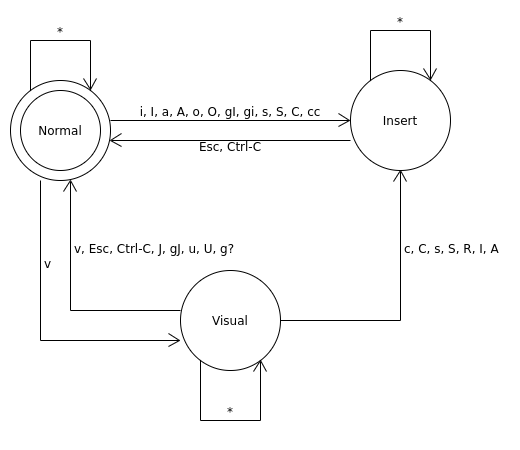
\includegraphics[width=0.8\textwidth]{images/FSM_simple_example.png}
			\caption{A simple example: FSM diagram}
		\end{figure}

		For the sake of simplicity, I took many liberties with the above diagram:
		\begin{itemize}
			\item{Instead of drawing a separate arrow for each transition, I condensed all key variations that start and go to the same state into a single arrow.}
			\item{Here the \verb|'*'| means "all other keys" and not the actual asterisk.}
			\item{Since this only contains a small subset of the actual modes, all transitions that go to undrawn states are also omitted.}
			\item{There are two kinds of problematic inputs both worth to discuss: \verb|Ctrl-C| and the likes of \verb|gi| and \verb|cc|.}
		\end{itemize}

		Multikey inputs such as \verb|Ctrl-C| are perfectly fine, because \verb|Ctrl| is only a modifier key and does not have any effect on its own (we can keep pressing \verb|Ctrl| anytime, nothing will happen). As a result, we can consider combinations like \verb|Ctrl-C| a unique (virtual) key. Note: capital letters are also in a similar boat, e.g. \verb|A| is technically \verb|Shift-a|.

		Inputs like \verb|gi| and \verb|cc| could be considered invalid if and only if we only allowed single keypresses to count as inputs, but, in fact, we can consider entire key sequences as input for any transition. It will not create ambiguity, because \verb|gi| and \verb|gI|, despite having the same prefix, are not equal. We do not need to introduce additional intermediate modes to handle such cases. Whenever we press a key which needs some follow-up key(s) to determine its action, nvim always waits for those follow-up key(s). At test execution, we can simply feed nvim the \verb|c| key twice in a row for example.

		Darcy Parker created a comprehensive diagram \cite{darcy-parker-diagram} that lists all states and transitions, albeit it was created in 2012 and for regular Vim, not Neovim. Still, his work matches our expected model in 99\%.

	\subsection{Creating the model}

		\textbf{Simple example}\\

		I used Model >> Test >> Relax \cite{relax}, an open source MBT framework developed at ELTE. It takes the FSM specification in JSON format as input and it can run various test generation algorithms on it. Here is the model for the small example discussed above:

		\begin{figure}[h]
			\centering
			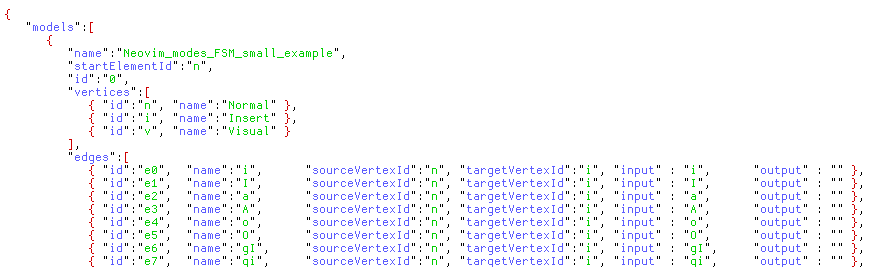
\includegraphics[width=1\textwidth]{images/Neovim_modes_FSM_small_example_partial.png}
			\caption{A simple example: JSON input for MTR (not all edges are on the image)}
		\end{figure}

		Some key notes:
		\begin{itemize}
			\item{I used the abbreviated mode characters from nvim's manual as state ids (n, i, v).}
			\item{The modes' full names are written for state names.}
			\item{Edge ids can simply be unique numbered keys.}
			\item{I have given the same name to the transitions as the input they take.}
			\item{We do not need to define any output, because we will be able to query the current mode (state) at any given time in the tests (discussed later). Differentiating between the states will not be a problem.}
		\end{itemize}

		{\parindent0pt
		\textbf{Actual model}\\
		}

		I did not include all 34 modes of nvim in the actual model for a number of reasons:
		\begin{itemize}
			\item{This project is intended to be more of a proof of concept or a case study, than a fully comprehensive testing of nvim.}
			\item{There are many "pseudo modes" like the different \verb|Operator Pending| ones. They can be accessed by pressing a key that starts an \textit{action}, then nvim waits for a \textit{motion} key, or series of keys that count as a motion. This would give us countless cases of different action-motion combinations, even if we ignore all negative cases where the action is not followed by a proper motion. It would be possible to extend the FSM to cover all these, but fully specifying all possible transitions for all possible keys with all operators would require a considerable amount of effort in itself. However, it could be a future improvement.}
			\item{For similar reasons, I also omitted more obscure and harder to test states like the \verb|Insert Completion| one or \verb|Special Character Pending|.}
			\item{If we really wanted to be pedantic, there would be an infinite number of states for some scenarios. For example, if we enter \verb|Ex| mode, we get a prompt which we can only exit by typing \verb|vi<CR>|. However, this only works if the prompt is empty beforehand, otherwise things like \verb|arbitrary-text-vi<CR>| won't leave the mode.}
		\end{itemize}

		The used FSM covers the following nine modes:

		\begin{figure}[h]
			\centering
			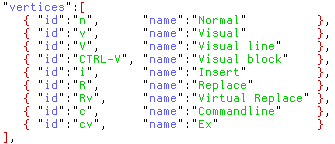
\includegraphics[width=0.5\textwidth]{images/vertices.png}
			\caption{States of our model}
		\end{figure}

		In order to fill the JSON file with all transitions, I defined a simpler TSV format which I preprocess with an awk one-liner. The format (which also accepts hashmarked lines as comments):\\

		\verb|<FROM-STATE> Tab <KEYS> Tab <TO-STATE>|\\

		\begin{figure}[h]
			\centering
			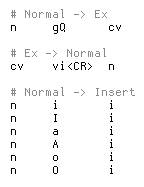
\includegraphics[width=0.25\textwidth]{images/transitions_tsv.png}
			\caption{Portion from transitions.tsv}
		\end{figure}

		And the awk command that turns this format into the JSON lines for MTR:\\

		{\parindent0pt
		\verb|$ awk '/^[^#]/ {|
		\verb|print "{ \"id\":\"e",n++,"\", \"name\":\"",$2,"\", |\\
		\verb|\"sourceVertexId\":\"",$1,"\", \"targetVertexId\":\"",$3,"\",|\\
		\verb|\"input\":\"",$2,"\", \"output\":\"\" },"|
		\verb|}' OFS= transitions.tsv|\\
		}

		\begin{figure}[h]
			\centering
			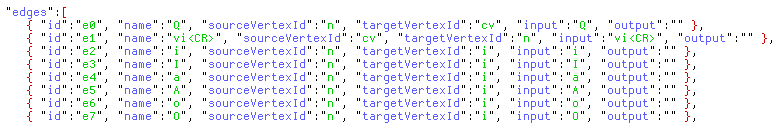
\includegraphics[width=1.0\textwidth]{images/transitions_json_lines_snippet.png}
			\caption{Generated JSON lines for the above transitions}
		\end{figure}

		The MBT framework can also visualize the model by adding the \verb|--graphviz| \cite{graphviz} option. This outputs a .dot file from which we can generate images:\\

		{\parindent0pt
		\verb|$ dot -Tpng Neovim_modes_FSM.dot > graphviz_model.png|\\
		\verb|$ dot -Tpng Neovim_modes_FSM-augmented.dot > graphviz_model_Eulerian.png|\\
		}

		Note: I also added the \verb|ratio=1.0;| line to the .dot files so the images' widths and heights are about the same.

		The below image is attached at \verb|images/graphviz_model.png|.\\There is also \verb|images/graphviz_model_Eulerian.png|, which depicts the Eulerian-augmented graph that MTR generated. Most algorithms require the FSM to have an Euler path (path touching every edge exactly once).

		\begin{figure}[h]
			\centering
			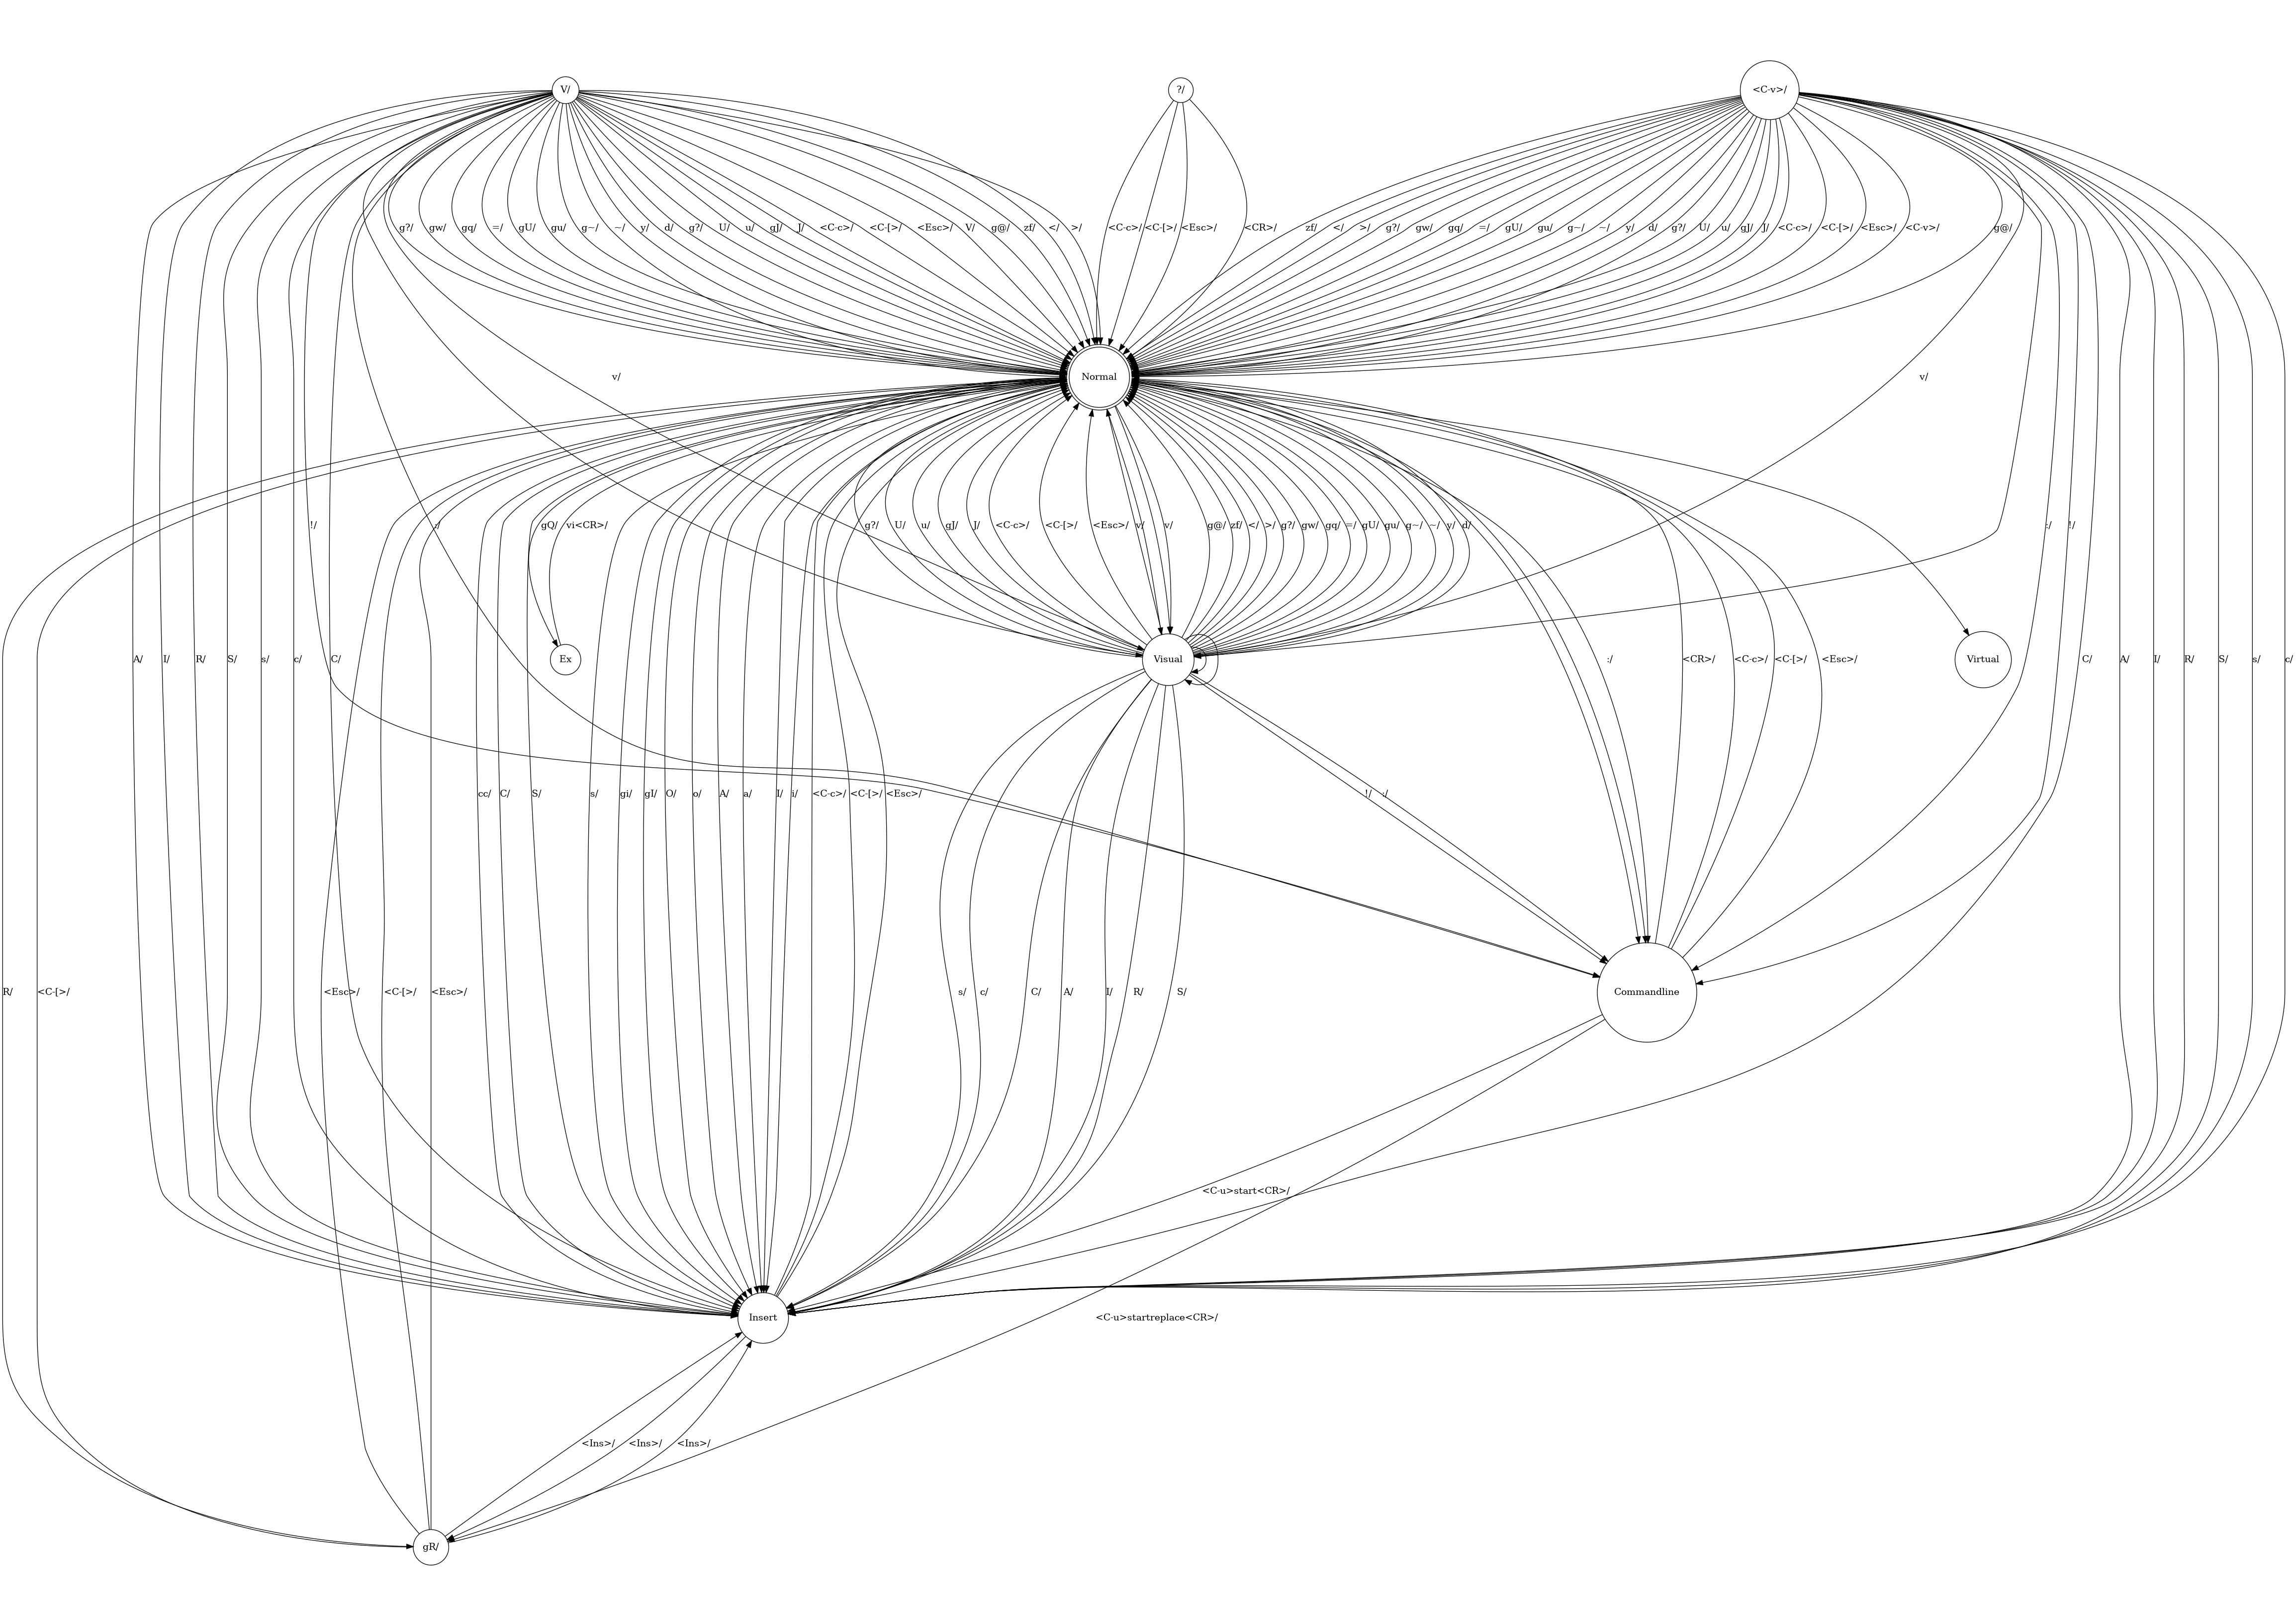
\includegraphics[width=1.0\textwidth]{images/graphviz_model.png}
			\caption{Base model generated by MTR using graphviz}
		\end{figure}

	\section{Test generation}

		Now that Neovim\_modes\_FSM.json is complete, we can run MBT algorithms on it using the MTR framework: Random walk \cite{random}, Transition Tour (TT) \cite{tt} and All-Transition-State (ATS) \cite{ats}.\\

		{\parindent0pt
		\verb|$ ./MTR -m Random -f Neovim_modes_FSM.json --pretty_json|\\
		\verb|$ ./MTR -m TT     -f Neovim_modes_FSM.json --pretty_json|\\
		\verb|$ ./MTR -m ATS    -f Neovim_modes_FSM.json --pretty_json|\\
		}

		The TT method generated the shortest test sequence: 274 inputs (which includes mostly single keypresses and some 2-3 long keystrokes) is enough to traverse all transitions.

		Random walk generates random inputs until it reaches its stopping condition. This condition was set to be 100\% transition coverage. (I ran the algorithm a couple of times, the resulting input sequence was always around 8000-11000 in length). The TT method was run with 100\% state- and transition coverage. ATS also guarantees covering all transitions. So the tests will cover all possible mode changes that we included in our model. Using these input sequences, we will be able to run automated tests to verify if all transitions are correct.

		\begin{table}[h!]
		\begin{center}
			\begin{tabular}{l|l|l|p{30mm}|l}
			\textbf{Algorithm} & \textbf{Runtime} & \textbf{Test suite size} & \textbf{Test sequence length} & \textbf{Summary}\\
			\hline
			Random walk & 0.022228 s & 434 KB & 8183 & rand\_result.csv\\
			\hline
			TT & 0.042106 s & 15 KB & 274 & tt\_result.csv\\
			\hline
			ATS & 0.096331 s & 35 KB & 652 & ats\_result.csv\\
			\hline
		\end{tabular}
		\caption{MBT algorithm runs and resulting test suites}
		\end{center}
		\end{table}

		\begin{figure}[!h]
			\centering
			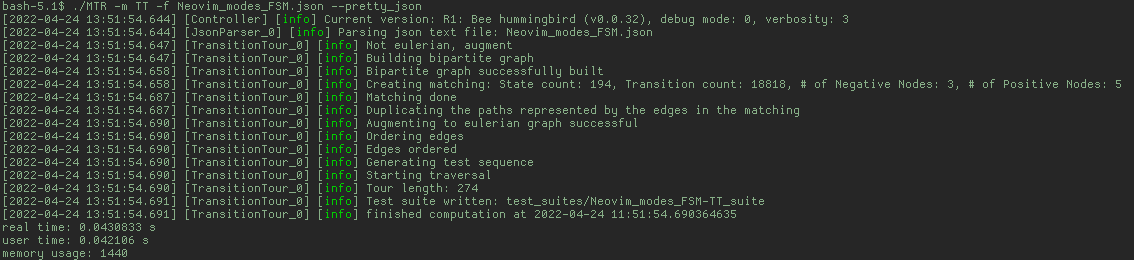
\includegraphics[width=1.0\textwidth]{images/TT_run.png}
			\caption{Running the TT method with the MBT framework}
		\end{figure}

		\begin{figure}[!h]
			\centering
			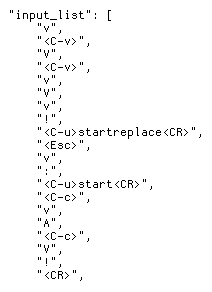
\includegraphics[width=0.35\textwidth]{images/test_input_sequence.png}
			\caption{Start of the test input sequence generated by the TT method\\It starts with checking the transitions between the three Visual modes}
		\end{figure}

\section{Test execution}

	There are two special commands that transition from \verb|Cmdline| to other modes: \verb|start<CR>| and \verb|startreplace<CR>|. Initial testing revealed a problem with them: we can reach \verb|Cmdline| from any of the \verb|Visual| modes by pressing \verb|:| or even \verb|!|. In this case, nvim adds the selection indicating prefix to the command: \verb|:'<,'>|. However, if we insert either of the above commands, we will get a prompt like \verb|:'<,'>start<CR>|, which, instead of switching mode, will only throw an error. Solution: I added a \verb|<C-u>| prefix to these transitions, i.e., \verb|<C-u>start<CR>| and \verb|<C-u>startreplace<CR>|. \verb|<C-u>| deletes all text till the beginning of the prompt. This solves a more general problem: no matter what got inserted to the command prompt so far, these two corrected keystrokes will always transition correctly.

	Another issue was that the two search keys \verb|/| and \verb|?| transition to \verb|Cmdline| mode and the above two commands will not work with them, not even with the \verb|<C-u>| prefix. The only solution is to introduce a new virtual mode to our model: "Cmdline search" (with id="cs"). But how can we differentiate this from regular \verb|Cmdline|, when nvim's \verb|mode()| function only returns 'c' for both? Luckily, nvim has another function called \verb|getcmdtype()|, which tells us what type of cmdline we currently have. Now our FSM has 10 states.

	\subsection{Test environment}

	{\parindent0pt
	\textbf{OS:} x86\_64 GNU/Linux 5.15.32-1-MANJARO\\
	\textbf{SUT:} NVIM v0.7.0, Build type: Release\\
	\textbf{Tools:} GNU Awk 5.1.1; Python 3.10.4; MTR version R1: Bee hummingbird (v0.0.32)
	}

	\subsection{Adaptation code}

		\subsubsection{Remote controlling Neovim}

			For the test execution, we can utilize nvim's remote controlling capabilities. It provides an API \cite{nvim-api} for running RPC calls through a TCP socket.

			In order to easily connect and use this API from a Python script, we must first install the \verb|Pynvim| package:\\

			\verb|$ pip3 install pynvim|\\

			The next step is to start nvim with its \verb|--listen| option. In this example, it will listen for calls at port 10000 of localhost:\\

			\verb|$ nvim -u NONE --listen 127.0.0.1:10000|\\

			Note: the \verb|-u NONE| option makes nvim ignore any startup configuration (e.g. .vimrc file) and it also does not load any plugins. This way, we can make sure that the SUT is truly a vanilla nvim instance and no user configurion or plugin will distort the test results. (For example, the user config could easily remap keys from their defaults which would lead to false results).

			Now we can connect to the API from python with the following lines:\\

			{\parindent0pt
			\verb|>>> from pynvim import attach|\\
			\verb|>>> nvim = attach("tcp", address="127.0.0.1", port=10000)|\\
			}

			We will use three nvim functions:

			\begin{itemize}
				\item{\verb|call:| We can call nvim's internal "mode()" function, which returns the string that represents the current mode.}
				\item{\verb|feedkeys:| Simulates keypresses as if they were feeded to nvim directly from the keyboard.}
				\item{\verb|replace_termcodes:| Needs to be used in conjunction with \verb|feedkeys| so nvim's key representations - also used in our model - get translated to proper terminal codes, e.g. \verb|<Esc>| to \verb|\x1b|.}
			\end{itemize}

			For example, to check if nvim starts in \verb|Normal| mode, then by pressing \verb|i| it goes to \verb|Insert|, then back to \verb|Normal| with \verb|<Esc>|, we can use the code snippet below:\\

			{\parindent0pt
			\verb|>>> nvim.call('mode') == 'n'|\\
			\verb|>>> nvim.feedkeys('i')|\\
			\verb|>>> nvim.call('mode') == 'i'|\\
			\verb|>>> nvim.feedkeys(nvim.replace_termcodes("<Esc>"))|\\
			\verb|>>> nvim.call('mode') == 'n'|
			}

		\subsubsection{The testing script}

		The script is named \texttt{test\_exec.py}, its short manual reads as follows:

		\begin{figure}[!h]
			\centering
			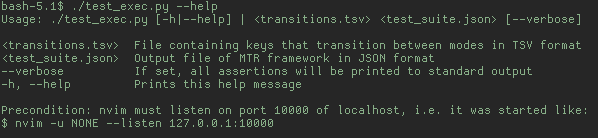
\includegraphics[width=1\textwidth]{images/test_exec_help.png}
			\caption{Running the script with the \texttt{-h} or \texttt{---help} option}
		\end{figure}

		Its first argument must be the transitions.tsv we used to generate the model and the second must be MTR's test suite output.

		After parsing its input files, it connects to the running nvim instance. Then it iterates over the test suite's \texttt{input\_list} and feeds each key sequence in it to the SUT. Before and after feeding each input, it queries nvim's current mode and then it checks whether we arrived to the correct destination mode based on the specification from transitions.tsv.

		Finally, it writes a test report that contains statistics about the number of assertions (total, ok, failed), the success rate and the execution time. If the \texttt{---verbose} option is set, it also outputs all assertions.

	\subsection{Test results}

		\begin{figure}[!h]
			\centering
			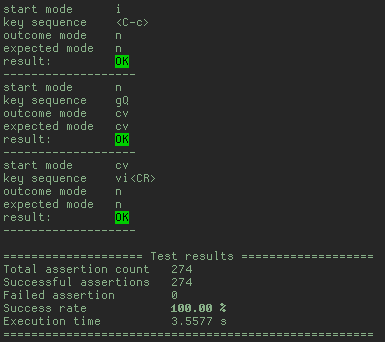
\includegraphics[width=0.5\textwidth]{images/test_exec_run_TT.png}
			\caption{Part of the verbose output of \texttt{test\_exec.py} on the TT generated test suite}
		\end{figure}

		\begin{table}[h!]
		\begin{center}
			\begin{tabular}{l|l|l||l|l|l}
			\textbf{Algorithm} & \textbf{Runtime} & \textbf{No. assertions} & \textbf{Passed} & \textbf{Failed} & \textbf{Success rate}\\
			\hline
			Random walk & 25.7596 s & 8183 & 8173 & 10 & 99.88 \%\\
			\hline
			TT & 3.5577 s & 274 & 274 & 0 & 100 \%\\
			\hline
			ATS & 10.2623 s & 652 & 652 & 0 & 100 \%\\
			\hline
		\end{tabular}
		\caption{Test execution results}
		\end{center}
		\end{table}

		%\begin{figure}[!h]
		%	\centering
		%	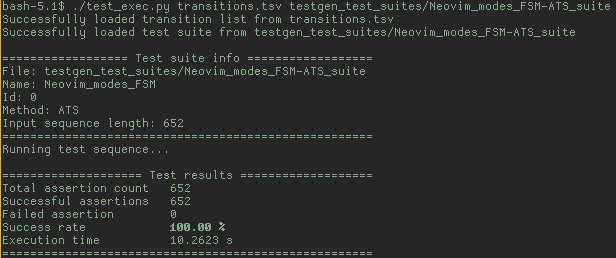
\includegraphics[width=0.8\textwidth]{images/test_exec_run_ATS.png}
		%	\caption{Output of \texttt{test\_exec.py} on the ATS generated test suite}
		%\end{figure}
		The test suites generated by TT and ATS both fully passed the tests. The Random walk method's input threw 10 failed assertions out of 8183. This proves that the Random method, despite it being inefficient, can be useful for revealing defects the other methods failed to catch. But if the other two method also covered all transitions, how could a failure happen with the Random walk? The problem hides in the model. There is a case where a transition needs a longer state history, then solely its preceding mode, i.e., at A->B->C, what C should be not only depends on B, but also A. All ten failed assertions are the same problem: from both \verb|Replace| and \verb|Virtual Replace|, we can press the \verb|<Ins>| key to enter \verb|Insert| mode, then \verb|<Ins>| again to return to where we came from. So if we transitioned from simple \verb|Replace|, we return there, if we came from \verb|Virtual Replace|, then we return there. Neovim remembers which replace mode it came from. There could be two ways to fix this:

		\begin{itemize}
			\item{Extend the model with a new mode, e.g. \verb|Insert-coming-from-Rv|. It should work exactly like \verb|Insert|, with the only difference being that on \verb|<Ins>| it would go to \verb|Virtual Replace| instead of \verb|Replace|.}
			\item{Augment the FSM to an EFSM (Extended Finite State Machine) with a variable that can tell us if we came from a replace mode to \verb|Insert| and if yes, which one. The MTR framework could convert the EFSM to an FSM for us with a command like: \verb|$ ./MTR -o conversion -m efsm_to_fsm -f Neovim_modes_EFSM.json --efsm| Once we got to the FSM, the workflow would be the same. This solution would be more laboursome, but maybe going for an EFSM model could prove useful in the long-run for similar technicalities.}
		\end{itemize}

		\begin{figure}[!h]
			\centering
			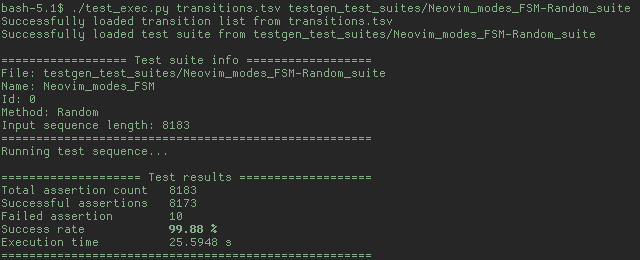
\includegraphics[width=0.8\textwidth]{images/test_exec_run_Random.png}
			\caption{Output of \texttt{test\_exec.py} on the Random walk generated test suite}
		\end{figure}

		\begin{figure}[!h]
			\centering
			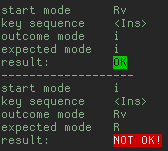
\includegraphics[width=0.25\textwidth]{images/test_exec_NOT_OK.png}
			\caption{Failed assertion in the Random walk}
		\end{figure}

		\newpage

\section{Future work}

	There are several ways to extend or improve this test solution:

	\begin{itemize}
		\item{Cover all 34 modes of nvim and all transitions between them.}
		\item{Add all reflexive transitions by defining a comprehensive set of key inputs. We would only need to write out all key inputs only once, because the MTR framework can fill up the rest of the unspecified transitions with loops using the \texttt{-o conversion -m ps\_to\_cs} options.}
		\item{The MTR tool could be further utilized. We could run other MBT methods like ATT or HSI, or we could even use the framework for injecting random faults to the model to check how good are the testcases in detecting all defects.}
		\item{Outlook: some techniques (e.g. use of the RPC API) could be applied to test other aspects of nvim too. For example, to test where different motions move the cursor, or how different actions affect the buffer. These do not align so naturally with an FSM model, but it may still be possible to translate these problems to some extent.}
	\end{itemize}

\section{Conclusion}

	This study has introduced readers to translating software behavior to a finite state machine, constructing a model from it, generating executable testcases through different MBT methods with the MTR framework, and successfully running and evaluating these tests using API calls and minimal logic in a small script.

	The example shows that model based approaches to test generation and automatic test execution can greatly reduce the amount of manual work. The only hand-written part of the entire testing workflow, besides the script, is the initial transitions.tsv file (214 lines of simple triples, a fully specified model for nvim would also probably be less than 1000 lines here).

	The lengths and runtimes of the resulted tests are also in an acceptable range. The longest taking 25 seconds to complete, I think it is safe to assume that running on even a fully specified model of nvim could be measured on the scale of minutes.

	Generated testcases and adaptation code like this could be used in regression testing nvim itself as well as similar software with minimal effort.

	\newpage

%-------------------------------- REFERENCES ----------------------------------

\begin{thebibliography}{1}
	\bibitem{nvim} Neovim homepage,\\https://neovim.io/ (2022.04.28)
	\bibitem{nvim-user-doc} Neovim's user manual,\\https://neovim.io/doc/user/ (2022.04.28)
	\bibitem{darcy-parker-diagram} Darcy Parker's Vim mode state diagram,\\https://gist.github.com/darcyparker/1886716 (2022.04.28)
	\bibitem{relax} Model >> Test >> Relax MBT framework,\\https://gitlab.inf.elte.hu/nga/ModelTestRelax (2022.04.28)
	\bibitem{graphviz} Graphviz homepage,\\https://graphviz.org/ (2022.04.28)
	\bibitem{random} Random walk method's documentation in MTR,\\https://gitlab.inf.elte.hu/nga/ModelTestRelax/\\-/blob/master/docs/user\_guide.md\#61-random-walk (2022.04.28)
	\bibitem{tt} Transition Tour method's documentation in MTR,\\https://gitlab.inf.elte.hu/nga/ModelTestRelax/\\-/blob/master/docs/user\_guide.md\#62-transition-tour (2022.04.28)
	\bibitem{ats} All-Transition-State method's documentation in MTR,\\https://gitlab.inf.elte.hu/nga/ModelTestRelax/\\-/blob/master/docs/user\_guide.md\#63-all-transition-state (2022.04.28)
	\bibitem{nvim-api} Neovim's API reference,\\https://neovim.io/doc/user/api.html (2022.04.28)
	\bibitem{pynvim} Pynvim's GitHub page,\\https://github.com/neovim/pynvim (2022.04.28)
\end{thebibliography}

\end{document}

